\documentclass[oneside]{book}
\usepackage[backend=biber,natbib=true,style=authoryear]{biblatex}
\addbibresource{/home/hong/1_NQBH/reference/bib.bib}
\usepackage[utf8]{vietnam}
\usepackage{tocloft}
\renewcommand{\cftsecleader}{\cftdotfill{\cftdotsep}}
\usepackage[colorlinks=true,linkcolor=blue,urlcolor=red,citecolor=magenta]{hyperref}
\usepackage{amsmath,amssymb,amsthm,mathtools,float,graphicx,algpseudocode,algorithm,tcolorbox,tikz,tkz-tab,subcaption}
\DeclareMathOperator{\arccot}{arccot}
\usepackage[inline]{enumitem}
\allowdisplaybreaks
\numberwithin{equation}{section}
\newtheorem{assumption}{Assumption}[section]
\newtheorem{nhanxet}{Nhận xét}[section]
\newtheorem{conjecture}{Conjecture}[section]
\newtheorem{corollary}{Corollary}[section]
\newtheorem{hequa}{Hệ quả}[section]
\newtheorem{definition}{Definition}[section]
\newtheorem{dinhnghia}{Định nghĩa}[section]
\newtheorem{example}{Example}[section]
\newtheorem{vidu}{Ví dụ}[section]
\newtheorem{lemma}{Lemma}[section]
\newtheorem{notation}{Notation}[section]
\newtheorem{principle}{Principle}[section]
\newtheorem{problem}{Problem}[section]
\newtheorem{baitoan}{Bài toán}[section]
\newtheorem{proposition}{Proposition}[section]
\newtheorem{menhde}{Mệnh đề}[section]
\newtheorem{question}{Question}[section]
\newtheorem{cauhoi}{Câu hỏi}[section]
\newtheorem{quytac}{Quy tắc}
\newtheorem{remark}{Remark}[section]
\newtheorem{luuy}{Lưu ý}[section]
\newtheorem{theorem}{Theorem}[section]
\newtheorem{tiende}{Tiên đề}[section]
\newtheorem{dinhly}{Định lý}[section]
\usepackage[left=0.5in,right=0.5in,top=1.5cm,bottom=1.5cm]{geometry}
\usepackage{fancyhdr}
\pagestyle{fancy}
\fancyhf{}
\lhead{\small \textsc{Sect.} ~\thesection}
\rhead{\small \nouppercase{\leftmark}}
\renewcommand{\sectionmark}[1]{\markboth{#1}{}}
\cfoot{\thepage}
\def\labelitemii{$\circ$}

\title{Some Topics in Elementary Mathematics\texttt{/}Grade 12}
\author{Nguyễn Quản Bá Hồng\footnote{Independent Researcher, Ben Tre City, Vietnam\\e-mail: \texttt{nguyenquanbahong@gmail.com}; website: \url{https://nqbh.github.io}.}}
\date{\today}

\begin{document}
\frontmatter
\maketitle
\setcounter{secnumdepth}{4}
\setcounter{tocdepth}{3}
\tableofcontents
\newpage

%------------------------------------------------------------------------------%

\mainmatter

\part{Đại Số \& Giải Tích -- Algebra \& Analysis}

\chapter{Ứng Dụng Đạo Hàm Để Khảo Sát \& Vẽ Đồ Thị của Hàm Số}

\begin{quotation}
	\textbf{Nội dung.} \textit{Ứng dụng đạo hàm \& giới hạn để xét 1 số tính chất quan trọng của hàm số \& đồ thị như: tính đơn điệu, cực trị, giá trị lớn nhất, giá trị nhỏ nhất của hàm số \& các đường tiệm cận của đồ thị; khảo sát sự biến thiên \& vẽ đồ thị của hàm số của 1 số hàm số đơn giản}.
\end{quotation}

\section{Tính Đơn Điệu của Hàm Số}
\textbf{Nội dung.} \textit{Ứng dụng đạo hàm để xét tính \emph{đơn điệu} (i.e., tính \emph{đồng biến} \& tính \emph{nghịch biến}) của hàm số}.

\begin{dinhnghia}[Hàm số đồng\texttt{/}nghịch biến]
	Giả sử $K$ là 1 khoảng, 1 đoạn hoặc 1 nửa khoảng \& $f$ là hàm số xác định trên $K$. Hàm số $f$ được gọi là \emph{đồng biến} trên $K$ nếu $\forall x_1,x_2\in K$, $x_1 < x_2\Rightarrow f(x_1) < f(x_2)$. Hàm số $f$ được gọi là \emph{nghịch biến} trên $K$ nếu $\forall x_1,x_2\in K$, $x_1 > x_2\Rightarrow f(x_1) < f(x_2)$.
\end{dinhnghia}
I.e., ``nếu hàm số $f$ xác định trên $K$ thì hàm số $f$ đồng biến trên $K$ khi \& chỉ khi với $x\in k$ tùy ý, ta có $\frac{f(x + \Delta x) - f(x)}{\Delta x} > 0$, $\forall\Delta x\ne 0$ mà $x + \Delta x\in K$; hàm số $f$ nghịch biến trên $K$ khi \& chỉ khi với $x\in K$ tùy ý, ta có $\frac{f(x + \Delta x) - f(x)}{\Delta x} < 0$, $\forall\Delta x\ne 0$ mà $x + \Delta x\in K$.'' -- \cite[p. 4]{SGK_Toan_12_giai_tich_nang_cao}

\begin{dinhly}
	Giả sử hàm số $f$ có đạo hàm trên khoảng $I$.
	\begin{enumerate*}
		\item[(a)] Nếu hàm số $f$ đồng biến trên khoảng $I$ thì $f'(x)\ge 0$, $\forall x\in I$.
		\item[(b)] Nếu hàm số $f$ nghịch biến trên khoảng $I$ thì $f'(x)\le 0$, $\forall x\in I$.
	\end{enumerate*}
\end{dinhly}
Đảo lại:

\begin{dinhly}
	\label{thm:dau dao ham & tinh dong bien}
	Giả sử hàm số $f$ có đạo hàm trên khoảng $I$.
	\begin{enumerate*}
		\item[(a)] Nếu $f'(x) > 0$, $\forall x\in I$ thì hàm số $f$ đồng biến trên khoảng $I$.
		\item[(b)] Nếu $f'(x) < 0$, $\forall x\in I$ thì hàm số $f$ nghịch biến trên khoảng $I$.
		\item[(c)] Nếu $f'(x) = 0$, $\forall x\in I$thì hàm số $f$ không đổi trên khoảng $I$.
	\end{enumerate*}
\end{dinhly}
Định lý trên cho ta 1 điều kiện đủ để hàm số đơn điệu trên 1 khoảng.

\begin{luuy}
	Khoảng $I$ trong định lý trên có thể được thay đổi bởi 1 đoạn hoặc 1 nửa khoảng. Khi đó phải bổ sung giả thiết ``Hàm số liên tục trên đoạn hoặc nửa khoảng đó''. E.g.:
	
	\begin{dinhly}
		Nếu hàm số $f$ liên tục trên đoạn $[a;b]$ \& có đạo hàm $f'(x) > 0$ trên khoảng $(a;b)$ thì hàm số $f$ đồng biến trên đoạn $[a;b]$.
	\end{dinhly}
	Người ta thường diễn đạt khẳng định này qua bảng biến thiên như sau:
	
	\begin{center}
		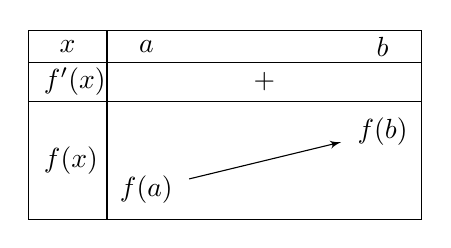
\begin{tikzpicture}
			\tkzTabInit
			[lgt=1,espcl=3] % tùy chọn
			{$x$/.4, $f’(x)$/.5, $f(x)$/1.5} % cột đầu tiên
			{$a$,$b$} % hàng 1 cột 2
			\tkzTabLine{,+,} % hàng 2 cột 2
			\tkzTabVar{-/ $f(a)$ , +/ $f(b)$} % hàng 3 cột 2
		\end{tikzpicture}
	\end{center}
\end{luuy}
``Việc tìm các khoảng đồng biến \& nghịch biến của 1 hàm số còn được nói gọn là xét \textit{chiều biến thiên của hàm số} đó. Qua định lý đã nêu, ta thấy việc xét chiều biến thiên của 1 hàm số có đạo hàm có thể chuyển về việc xét dấu đạo hàm của nó.'' -- \cite[p. 5]{SGK_Toan_12_giai_tich_nang_cao}

Có thể mở rộng định lý \ref{thm:dau dao ham & tinh dong bien} như sau:

\begin{dinhly}
	Giả sử hàm số $f$ có đạo hàm trên khoảng $I$. Nếu $f'(x)\ge 0$, $\forall x\in I$ (hoặc $f'(x)\le 0$, $\forall x\in I$) \& $f'(x) = 0$ chỉ tại 1 số hữu hạn điểm của $I$ thì hàm số $f$ đồng biến (hoặc nghịch biến) trên $I$.
\end{dinhly}

%------------------------------------------------------------------------------%

\section{Cực Trị của Hàm Số}
\textbf{Nội dung.} \textit{Cực đại, cực tiểu của hàm số; quan hệ giữa cực đại, cực tiểu với dấu của đạo hàm cấp 1 \& đạo hàm cấp 2 của hàm số}.

\subsection{Khái niệm cực trị của hàm số}

\begin{dinhnghia}[Cực trị]
	``Giả sử hàm số $f$ xác định trên tập hợp $\mathcal{D}\subset\mathbb{R}$ \& $x_0\in\mathcal{D}$.
	\begin{enumerate*}
		\item[(a)] $x_0$ được gọi là 1 \emph{điểm cực đại} của hàm số $f$ nếu tồn tại 1 khoảng $(a;b)$ chứa điểm $x_0$ sao cho $(a;b)\subset\mathcal{D}$ \& $f(x) < f(x_0)$, $\forall x\in(a;b)\backslash\{x_0\}$. Khi đó $f(x_0)$ được gọi là \emph{giá trị cực đại} của hàm số $f$.
		\item[(b)] $x_0$ được gọi là 1 \emph{điểm cực tiểu} của hàm số $f$ nếu tồn tại 1 khoảng $(a;b)$ chứa điểm $x_0$ sao cho $(a;b)\subset\mathcal{D}$ \& $f(x) > f(x_0)$, $\forall x\in(a;b)\backslash\{x_0\}$. Khi đó $f(x_0)$ được gọi là \emph{giá trị cực tiểu} của hàm số $f$.
	\end{enumerate*}
	Điểm cực đại \& điểm cực tiểu được gọi chung là \emph{điểm cực trị}. Giá trị cực đại \& giá trị cực tiểu được gọi chung là \emph{cực trị}.
\end{dinhnghia}
Nếu $x_0$ là 1 điểm cực trị của hàm số $f$ thì người ta nói rằng hàm số $f$ đạt cực trị tại điểm $x_0$.'' -- \cite[p. 10]{SGK_Toan_12_giai_tich_nang_cao}

\begin{luuy}
	\begin{enumerate*}
		\item[(a)] ``Giá trị cực đại (cực tiểu) $f(x_0)$ của hàm số $f$ nói chung không phải là giá trị lớn nhất (nhỏ nhất) của hàm số $f$ trên tập hợp $\mathcal{D}$; $f(x_0)$ chỉ là giá trị lớn nhất (nhỏ nhất) của hàm số $f$ trên 1 khoảng $(a;b)$ nào đó chứa điểm $x_0$.
		\item[(b)] Hàm số $f$ có thể đạt cực đại hoặc cực tiểu tại nhiều điểm trên tập hợp $\mathcal{D}$. Hàm số cũng có thể không có cực trị trên 1 tập hợp số thực cho trước.
		\item[(c)] Đôi khi người ta cũng nói đến điểm cực trị của đồ thị.
	\end{enumerate*}
\end{luuy}
Nếu $x_0$ là 1 điểm cực trị của hàm số $f$ thì điểm $(x_0;f(x_0))$ được gọi là \textit{điểm cực trị của đồ thị} hàm số $f$.'' -- \cite[p. 11]{SGK_Toan_12_giai_tich_nang_cao}

\subsection{Điều kiện cần để hàm số đạt được cực trị}
``Quan sát đồ thị của hàm số $y = f(x)$, ta thấy nếu hàm số $f$ đạt cực trị tại điểm $x_0$ \& nếu đồ thị của hàm số có tiếp tuyến tại điểm $(x_0;f(x_0))$ thì tiếp tuyến đó song song với trục hoành, i.e., $f'(x_0) = 0$.

\begin{dinhly}
	Giả sử hàm số $f$ đạt cực trị tại điểm $x_0$. Khi đó, nếu $f$ có đạo hàm tại $x_0$ thì $f'(x_0) = 0$.
\end{dinhly}
``Điều ngược lại có thể không đúng. Đạo hàm $f'$ có thể bằng $0$ tại điểm $x_0$ nhưng hàm số không đạt cực trị tại điểm $x_0$. E.g., xét hàm số $f(x) = x^3$, ta có $f'(x) = 3x^2$ \& $f'(0) = 0$. Tuy nhiên, hàm số $f$ không đạt cực trị tại điểm $x = 0$. Thật vậy, vì $f'(x) > 0$, $\forall x\ne 0$ nên hàm số $f$ đồng biến trên $\mathbb{R}$.'' -- \cite[p. 11]{SGK_Toan_12_giai_tich_nang_cao}

\begin{luuy}
	``Hàm số có thể đạt cực trị tại 1 điểm mà tại điểm đó hàm số không có đạo hàm. E.g., hàm số $y = f(x) = |x|$ xác định trên $\mathbb{R}$. Vì $f(0) = 0$ \& $f(x) > 0$, $\forall x\ne 0$ nên hàm số đạt cực tiểu tại điểm $x = 0$. Dễ thấy hàm số $y = |x|$ không có đạo hàm tại điểm $x = 0$ (Fig. \ref{fig:graph_abs}).
	
	\begin{figure}[H]
		\centering
		\includegraphics[scale=0.15]{graph_abs}
		\caption{Đồ thị của hàm số $y = f(x) = |x|$, \cite[Hình 1.3, p. 12]{SGK_Toan_12_giai_tich_nang_cao}.}
		\label{fig:graph_abs}
	\end{figure}
	Như vậy, 1 hàm số chỉ có thể đạt cực trị tại 1 điểm mà tại đó đạo hàm của hàm số bằng $0$, hoặc tại đó hàm số không có đạo hàm.'' -- \cite[p. 11]{SGK_Toan_12_giai_tich_nang_cao}
\end{luuy}

\subsection{Điều kiện đủ để hàm số đạt cực trị}
``Định lý sau cho ta 1 điều kiện đủ để hàm số đạt cực trị.

\begin{dinhly}
	\label{thm:dieu kien du de ham so dat cuc tri}
	Giả sử hàm số $f$ liên tục trên khoảng $(a;b)$ chứa điểm $x_0$ \& có đạo hàm trên các khoảng $(a;x_0)$ \& $(x_0;b)$. Khi đó:
	\begin{enumerate*}
		\item[(a)] Nếu $f'(x) < 0$, $\forall x\in(a;x_0)$ \& $f'(x) > 0$, $\forall x\in(x_0;b)$ thì hàm số $f$ đạt cực tiểu tại điểm $x_0$.
		\item[(b)] Nếu $f'(x) > 0$, $\forall x\in(a;x_0)$ \& $f'(x) < 0$, $\forall x\in(x_0;b)$ thì hàm số $f$ đạt cực đại tại điểm $x_0$.
	\end{enumerate*}
\end{dinhly}
I.e.,
\begin{enumerate*}
	\item[(a)] Nếu $f'(x)$ đổi dấu từ âm sang dương khi $x$ qua điểm $x_0$  (theo chiều tăng) thì hàm số đạt cực tiểu tại điểm $x_0$.
	\item[(b)] Nếu $f'(x)$ đổi dấu từ dương sang âm khi $x$ qua điểm $x_0$ (theo chiều tăng) thì hàm số đạt cực đại tại điểm $x_0$.
\end{enumerate*}

\begin{proof}[Chứng minh]
	\begin{enumerate*}
		\item[(a)] Vì hàm số $f$ liên tục trên nửa khoảng $(a;x_0]$ \& $f'(x) < 0$, $\forall x\in(a;x_0)$ nên hàm số $f$ nghịch biến trên $(a;x_0]$. Do đó, $f(x) > f(x_0)$, $\forall x\in(a;x_0)$. Tương tự, vì hàm số $f$ liên tục trên nửa khoảng $[x_0;b)$ \& $f'(x) > 0$, $\forall x\in(x_0;b)$ nên hàm số đồng biến trên $[x_0;b)$. Do đó $f(x) > f(x_0)$, $\forall x\in(x_0;b)$. Vậy $f(x) > f(x_0)$, $\forall x\in(a;b)\backslash\{x_0\}$, i.e., hàm số $f$ đạt cực tiểu tại điểm $x_0$.
		\item[(b)] Chứng minh tương tự.
	\end{enumerate*}
\end{proof}
Định lý \ref{thm:dieu kien du de ham so dat cuc tri} được viết gọn lại trong 2 bảng biến thiên sau:

\begin{center}
	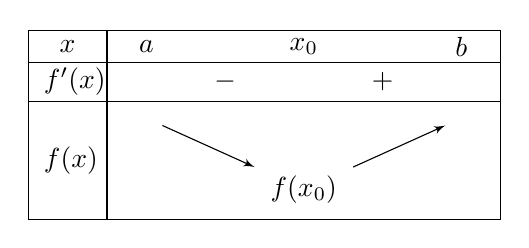
\begin{tikzpicture}
		\tkzTabInit
		[lgt=1,espcl=2] % tùy chọn
		{$x$/.4, $f’(x)$/.5, $f(x)$/1.5} % cột đầu tiên
		{$a$, $x_0$, $b$} % hàng 1 cột 2
		\tkzTabLine{,-,,+,} % hàng 2 cột 2
		\tkzTabVar{+/ , -/ $f(x_0)$ , +/ } % hàng 3 cột 2
	\end{tikzpicture}\hspace{1cm}
	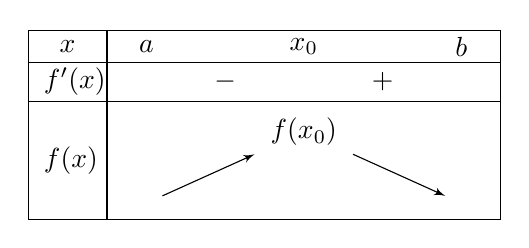
\begin{tikzpicture}
		\tkzTabInit
		[lgt=1,espcl=2] % tùy chọn
		{$x$/.4, $f’(x)$/.5, $f(x)$/1.5} % cột đầu tiên
		{$a$, $x_0$, $b$} % hàng 1 cột 2
		\tkzTabLine{,-,,+,} % hàng 2 cột 2
		\tkzTabVar{-/ , +/ $f(x_0)$ , -/ } % hàng 3 cột 2
	\end{tikzpicture}
\end{center}
Từ định lý \ref{thm:dieu kien du de ham so dat cuc tri} ta có quy tắc tìm cực trị sau đây.

\begin{quytac}
	\begin{enumerate*}
		\item Tìm $f'(x)$.
		\item Tìm các điểm $x_i$ tại đó đạo hàm của hàm số bằng $0$ hoặc hàm số liên tục nhưng không có đạo hàm.
		\item Xét dấu $f'(x)$. Nếu $f'(x)$ đổi dấu khi $x$ qua điểm $x_i$ thì hàm số đạt cực trị tại $x_i$.'' -- \cite[pp. 11--14]{SGK_Toan_12_giai_tich_nang_cao}
	\end{enumerate*}
\end{quytac}
``Có thể sử dụng đạo hàm cấp 2 để tìm cực trị của hàm số.

\begin{dinhly}
	\label{thm:dao ham cap 2 & cuc tri ham so}
	Giả sử hàm số $f$ có đạo hàm cấp 1 trên khoảng $(a;b)$ chứa điểm $x_0$, $f'(x_0) = 0$ \& $f$ có đạo hàm cấp 2 khác $0$ tại điểm $x_0$.
	\begin{enumerate*}
		\item[(a)] Nếu $f''(x_0) < 0$ thì hàm số $f$ đạt cực đại tại điểm $x_0$.
		\item[(b)] Nếu $f''(x_0) > 0$ thì hàm số $f$ đạt cực tiểu tại điểm $x_0$.
	\end{enumerate*}
\end{dinhly}
Từ định lý \ref{thm:dao ham cap 2 & cuc tri ham so}, ta có 1 quy tắc khác để tìm cực trị của hàm số (nếu hàm số có đạo hàm cấp 2).

\begin{quytac}
	\begin{enumerate*}
		\item Tìm $f'(x)$.
		\item Tìm các nghiệm $x_i$ của phương trình $f'(x) = 0$.
		\item Tìm $f''(x)$ \& tính $f''(x_i)$. Nếu $f''(x_i) < 0$ thì hàm số đạt cực đại tại điểm $x_i$. Nếu $f''(x_i) > 0$ thì hàm số đạt cực tiểu tại điểm $x_i$.'' -- \cite[pp. 15--16]{SGK_Toan_12_giai_tich_nang_cao}
	\end{enumerate*}
\end{quytac}

%------------------------------------------------------------------------------%

\section{Giá Trị Lớn Nhất \& Giá Trị Nhỏ Nhất của Hàm Số}
\textbf{Nội dung.} \textit{Các bài toán dẫn đến việc tìm giá trị lớn nhất \& giá trị nhỏ nhất của hàm số trên 1 tập hợp số thực cho trước, ứng dụng tính đơn điệu \& cực trị của hàm số để tìm giá trị lớn nhất \& giá trị nhỏ nhất của hàm số}.

\begin{dinhnghia}[Giá trị lớn\texttt{/}nhỏ nhất]
	``Giả sử hàm số $f$ xác định trên tập hợp $\mathcal{D}\subset\mathbb{R}$.
	\begin{enumerate*}
		\item[(a)] Nếu tồn tại 1 điểm $x_0\in\mathcal{D}$ sao cho $f(x)\le f(x_0)$, $\forall x\in\mathcal{D}$ thì số $M = f(x_0)$ được gọi là \emph{giá trị lớn nhất} của hàm số $f$ trên $\mathcal{D}$, ký hiệu là $M\coloneqq\max_{x\in\mathcal{D}} f(x)$.
		\item[(b)] Nếu tồn tại 1 điểm $x_0\in\mathcal{D}$ sao cho $f(x)\ge f(x_0)$, $\forall x\in\mathcal{D}$ thì số $m = f(x_0)$ được gọi là \emph{giá trị nhỏ nhất} của hàm số $f$ trên $\mathcal{D}$, ký hiệu là $m = \min_{x\in\mathcal{D}} f(x)$.
	\end{enumerate*}
\end{dinhnghia}
Như vậy, muốn chứng tỏ rằng số $M$ (hoặc $m$) là giá trị lớn nhất (hoặc giá trị nhỏ nhất) của hàm số $f$ trên tập hợp $\mathcal{D}$ cần chỉ rõ:
\begin{enumerate*}
	\item[(a)] $f(x)\le M$ (hoặc $f(x)\ge m$), $\forall x\in\mathcal{D}$.
	\item[(b)] Tồn tại ít nhất 1 điểm $x_0\in\mathcal{D}$ sao cho $f(x_0) = M$ (hoặc $f(x_0) = m$).
\end{enumerate*}
Ta quy ước rằng khi nói giá trị lớn nhất hay nhỏ nhất của hàm số $f$ (mà không nói ``trên tập $\mathcal{D}$'') thì ta hiểu đó là giá trị lớn nhất hay nhỏ nhất của $f$ trên tập xác định của nó.'' -- \cite[p. 18]{SGK_Toan_12_giai_tich_nang_cao}

``Phương pháp thường được sử dụng để tìm giá trị lớn nhất \& giá trị nhỏ nhất của hàm số trên 1 tập hợp là lập bảng biến thiên của hàm số trên tập hợp đó.'' -- \cite[p. 19]{SGK_Toan_12_giai_tich_nang_cao}

\begin{nhanxet}
	``Người ta đã chứng minh được rằng hàm số liên tục trên 1 đoạn thì đạt được giá trị lớn nhất \& nhỏ nhất trên đoạn đó. Trong nhiều trường hợp, có thể tìm giá trị lớn nhất \& giá trị nhỏ nhất của hàm số trên 1 đoạn mà không cần lập bảng biến thiên của nó.
\end{nhanxet}
Giả sử hàm số $f$ liên tục trên đoạn $[a;b]$ \& có đạo hàm trên khoảng $(a;b)$, có thể trừ 1 số hữu hạn điểm. Nếu $f'(x) = 0$ chỉ tại 1 số hữu hạn điểm thuộc $(a;b)$ thì ta có quy tắc tìm giá trị lớn nhất \& nhỏ nhất của hàm $f$ trên đoạn $[a;b]$ như sau:

\begin{quytac}
	\begin{enumerate*}
		\item Tìm các điểm $x_i\in(a;b)$, $i = 1,\ldots,m$, tại đó hàm số $f$ có đạo hàm bằng $0$ hoặc không có đạo hàm.
		\item Tính $f(x_i)$, $i = 1,\ldots,m$, $f(a)$, \& $f(b)$.
		\item So sánh các giá trị tìm được.
	\end{enumerate*}
	Số lớn nhất trong các giá trị đó là giá trị lớn nhất của $f$ trên đoạn $[a;b]$, số nhỏ nhất trong các gía trị đó là giá trị nhỏ nhất của $f$ trên đoạn $[a;b]$.'' -- \cite[p. 21]{SGK_Toan_12_giai_tich_nang_cao}
\end{quytac}

%------------------------------------------------------------------------------%

\section{Đồ Thị của Hàm Số \& Phép Tịnh Tiến Hệ Tọa Độ}
\textbf{Nội dung.} \textit{Phép tịnh tiến hệ tọa độ, nhờ đó có thể xác định được trục đối xứng \& tâm đối xứng của 1 số đường cong}.

\begin{dinhnghia}[Đồ thị của hàm số]
	``\emph{Đồ thị của hàm số} $y = f(x)$ xác định trên tập $\mathcal{D}$ là tập hợp tất cả các điểm $(x;f(x))$, $x\in\mathcal{D}$ của mặt phẳng tọa độ.
\end{dinhnghia}
Người ta còn gọi đồ thị của hàm số $y = f(x)$ là \textit{đường cong có phương trình là $y = f(x)$} (gọi tắt là \textit{đường cong} $y = f(x)$). Trong nhiều trường hợp việc thay hệ tọa độ đã có bởi 1 hệ tọa độ mới giúp ta nghiên cứu đường cong thuận tiện hơn.'' -- \cite[p. 24]{SGK_Toan_12_giai_tich_nang_cao}

\subsection{Phép tịnh tiến hệ tọa độ \& công thức chuyển hệ tọa độ}
``Giả sử $I$ là 1 điểm của mặt phẳng \& $(x_0;y_0)$ là tọa độ của điểm $I$ đối với hệ tọa độ $Oxy$. Gọi $IXY$ là hệ tọa độ mới có gốc là điểm $I$ \& 2 truc $IX,IY$ theo thứ tự có cùng các vector đơn vị $\vec{i},\vec{j}$ với 2 trục $Ox,Oy$ (Fig. \ref{fig:2_he_truc_toa_do}).

\begin{figure}[H]
	\centering
	\includegraphics[scale=0.13]{2_he_truc_toa_do}
	\caption{2 hệ trục tọa độ, \cite[Hình 1.5, p. 25]{SGK_Toan_12_giai_tich_nang_cao}.}
	\label{fig:2_he_truc_toa_do}
\end{figure}
Giả sử $M$ là 1 điểm bất kỳ của mặt phẳng. Gọi $(x;y)$ là tọa độ của điểm $M$ đối với hệ tọa độ $Oxy$ \& $(X;Y)$ là tọa độ của điểm $M$ đối với hệ tọa độ $IXY$. Khi đó: $\overrightarrow{OM} = \overrightarrow{OI} + \overrightarrow{IM}$ hay $x\vec{i} + y\vec{j} = (x_0\vec{i} + y_0\vec{j}) + (X\vec{i} + Y\vec{j}) = (X + x_0)\vec{i} + (Y + y_0)\vec{j}$. Do đó $(x = X + x_0)\land(y = Y + y_0)$. Các hệ thức trên gọi là \textit{công thức chuyển hệ tọa độ} trong phép tịnh tiến theo vector $\overrightarrow{OI}$.'' -- \cite[p. 25]{SGK_Toan_12_giai_tich_nang_cao}

\subsection{Phương trình của đường cong đối với hệ tọa độ mới}
``Giả sử $(\mathcal{G})$\footnote{Ký hiệu $\mathcal{G}$ được lấy từ chữ cái đầu của từ \textit{graph}, i.e., đồ thị.} là đồ thị\footnote{\textbf{graph} [n] a diagram, consisting of a line or lines, showing the relation between 2 or more sets of numbers.} của hàm số $y = f(x)$ đối với hệ tọa độ $Oxy$ đã cho. Khi đó phương trình của đường cong $(\mathcal{G})$ đối với hệ tọa độ $Oxy$ là $y = f(x)$. Ta sẽ viết phương trình của $(\mathcal{G})$ đối với hệ tọa độ mới $IXY$. Giả sử $M$ là 1 điểm bất kỳ của mặt phẳng, $(x;y)$ \& $(X;Y)$ là tọa độ của điểm $M$, theo thứ tự, đối với hệ tọa độ $Oxy$ \& $IXY$. Khi đó: $M\in(\mathcal{G})\Leftrightarrow y = f(x)$. Áp dụng công thức chuyển hệ tọa độ trong phép tịnh tiến theo vector $\overrightarrow{OI}$, ta có $M\in(\mathcal{G})\Leftrightarrow Y + y_0 = f(X + x_0)\Leftrightarrow Y = f(X + x_0) - y_0$. Vậy phương trình của đường cong $\mathcal{G}$ đối với hệ tọa độ $IXY$ là $Y = f(X + x_0) - y_0$.'' -- \cite[pp. 25--26]{SGK_Toan_12_giai_tich_nang_cao}

%------------------------------------------------------------------------------%

\section{Đường Tiệm Cận của Đồ Thị Hàm Số}

\subsection{Đường tiệm cận đứng \& đường tiệm cận ngang}
``Ta đã biết đồ thị của hàm số $f(x) = \frac{1}{x}$ là đường hyperbĐol gồm 2 nhánh nằm trong góc phần 4 thứ nhất \& thứ 3 của mặt phẳng tọa độ.

\begin{figure}[H]
	\centering
	\includegraphics[scale=0.13]{hyperbol}
	\caption{Đồ thị của hàm số $f(x) = \frac{1}{x}$, \cite[Hình 1.6, p. 28]{SGK_Toan_12_giai_tich_nang_cao}.}
	\label{fig:hyperbol}
\end{figure}
Ta có: $\lim_{x\to+\infty} f(x) = \lim_{x\to+\infty} \frac{1}{x} = 0$, $\lim_{x\to-\infty} f(x) = \lim_{x\to-\infty} \frac{1}{x} = 0$. I.e., khoảng cách $MH = |f(x)|$ từ điểm $M$ của đồ thị đến trục hoành dần đến $0$ khi điểm $M$ theo đường hyperbol đi xa ra vô tận về phía phải hoặc phía trái. Người ta gọi trục hoành là đường tiệm cận ngang của đồ thị hàm số $y = \frac{1}{x}$. Ta cũng có: $\lim_{x\to 0^+} f(x) = \lim_{x\to 0^+} \frac{1}{x} = +\infty$ \& $\lim_{x\to 0^-} f(x) = \lim_{x\to 0^-} \frac{1}{x} = -\infty$. I.e., khoảng cách $NK = |x|$ từ 1 điểm $N$ của đồ thị đến trục tung dần đến $0$ khi điểm $N$ theo đồ thị đi xa ra vô tận về phía trên hoặc phía dưới. Người ta gọi trục tung là \textit{đường tiệm cận đứng} của đồ thị hàm số $y = \frac{1}{x}$. 1 cách tổng quát, ta có:

\begin{dinhnghia}[Tiệm cận ngang]
	Đường thẳng $y = y_0$ được gọi là \emph{đường tiệm cận ngang} (gọi tắt là \emph{tiệm cận ngang}) của đồ thị hàm số $y = f(x)$ nếu $\lim_{x\to+\infty} f(x) = y_0$ hoặc $\lim_{x\to-\infty} f(x) = y_0$.
\end{dinhnghia}

\begin{figure}[H]
	\centering
	\begin{subfigure}{.5\textwidth}
		\centering
		\includegraphics[width=.5\linewidth]{tiem_can_ngang_a}
		\caption{Đường thẳng $y = y_0$ là tiệm cận ngang của đồ thị (khi $x\to+\infty$).}
	\end{subfigure}%
	\begin{subfigure}{.5\textwidth}
		\centering
		\includegraphics[width=.5\linewidth]{tiem_can_ngang_b}
		\caption{Đường thẳng $y = y_0$ là tiệm cận ngang của đồ thị (khi $x\to-\infty$).}
	\end{subfigure}
	\caption{Tiệm cận ngang của đồ thị, \cite[Hình 1.7, p. 29]{SGK_Toan_12_giai_tich_nang_cao}.}
	\label{fig:tiem_can_ngang}
\end{figure}

\begin{dinhnghia}[Tiệm cận đứng]
	Đường thẳng $x = x_0$ được gọi là \emph{đường tiệm cận đứng} (gọi tắt là \emph{tiệm cận đứng}) của đồ thị hàm số $y = f(x)$ nếu ít nhất 1 trong các điều kiện sau được thỏa mãn: $\lim_{x\to x_0^-} f(x) = +\infty$, $\lim_{x\to x_0^+} f(x) = +\infty$, $\lim_{x\to x_0^-} f(x) = -\infty$, $\lim_{x\to x_0^+} f(x) = -\infty$.'' -- \cite[pp. 28--30]{SGK_Toan_12_giai_tich_nang_cao}
\end{dinhnghia}

\begin{figure}[H]
	\centering
	\begin{subfigure}{.5\textwidth}
		\centering
		\includegraphics[width=.5\linewidth]{tiem_can_dung_a}
		\caption{}
	\end{subfigure}%
	\begin{subfigure}{.5\textwidth}
		\centering
		\includegraphics[width=.5\linewidth]{tiem_can_dung_b}
		\caption{}
	\end{subfigure}
	\begin{subfigure}{.5\textwidth}
		\centering
		\includegraphics[width=.5\linewidth]{tiem_can_dung_c}
		\caption{}
	\end{subfigure}%
	\begin{subfigure}{.5\textwidth}
		\centering
		\includegraphics[width=.5\linewidth]{tiem_can_dung_d}
		\caption{}
	\end{subfigure}
	\caption{(a) \& (c) Đường thẳng $x = x_0$ là tiệm cận đứng của đồ thị (khi $x\to x_0^-$), (b) \& (d) Đường thẳng $x = x_0$ là tiệm cận đứng của đồ thị (khi $x\to x_0^+$), \cite[Hình 1.8, p. 30]{SGK_Toan_12_giai_tich_nang_cao}.}
	\label{fig:tiem_can_dung}
\end{figure}

\subsection{Đường tiệm cận xiên}
``Cho $(\mathcal{C})$ là đồ thị của hàm số $y = f(x)$ \& $(d)$ là đường thẳng $y = ax + b$ ($a\ne 0$). Gọi $M$ \& $N$ là 2 điểm của $(\mathcal{C})$ \& $(d)$ có cùng hoành độ $x$ (Fig. \ref{fig:tiem_can_xien}).

\begin{figure}[H]
	\centering
	\begin{subfigure}{.5\textwidth}
		\centering
		\includegraphics[width=.6\linewidth]{tiem_can_xien_a}
		\caption{Đường thẳng $y = ax + b$ là tiệm cận xiên của đồ thị (khi $x\to+\infty$).}
	\end{subfigure}%
	\begin{subfigure}{.5\textwidth}
		\centering
		\includegraphics[width=.5\linewidth]{tiem_can_xien_b}
		\caption{Đường thẳng $y = ax + b$ là tiệm cận xiên của đồ thị (khi $x\to-\infty$).}
	\end{subfigure}
	\caption{Tiệm cận xiên của đồ thị, \cite[Hình 1.11, p. 33]{SGK_Toan_12_giai_tich_nang_cao}.}
	\label{fig:tiem_can_xien}
\end{figure}
Nếu độ dài của đoạn thẳng $MN$ dần đến $0$ khi $x$ dần đến $+\infty$ (hoặc khi $x$ dần đến $-\infty$) thì đường thẳng $(d)$ được gọi là \textit{đường tiệm cận xiên} của $(\mathcal{C})$. Vì $MN = |f(x) - (ax + b)|$ nên ta có định nghĩa sau:

\begin{dinhnghia}[Tiệm cận xiên]
	\label{def:tiem can xien}
	Đường thẳng $y = ax + b$, $a\ne 0$, được gọi là \emph{đường tiệm cận xiên} (gọi tắt là \emph{tiệm cận xiên}) của đồ thị hàm số $y = f(x)$ nếu $\lim_{x\to+\infty} [f(x) - (ax + b)] = 0$, hoặc $\lim_{x\to-\infty} [f(x) - (ax + b)] = 0$.'' -- \cite[p. 32]{SGK_Toan_12_giai_tich_nang_cao}
\end{dinhnghia}

\begin{luuy}
	``Để xác định các hệ số $a,b$ trong phương trình của đường tiệm cận xiên, ta có thể áp dụng các công thức sau: $a = \lim_{x\to+\infty} \frac{f(x)}{x}$, $b = \lim_{x\to+\infty} [f(x) - ax]$, hoặc $a = \lim_{x\to-\infty} \frac{f(x)}{x}$, $b = \lim_{x\to-\infty} [f(x) - ax]$. (Khi $a = 0$ thì ta có tiệm cận ngang).
\end{luuy}

\begin{proof}[Chứng minh]
	Thật vậy, xét trường hợp $x\to+\infty$, giả sử hàm số $f$ xác định trên khoảng $(\alpha;+\infty)$ \& đường thẳng $y = ax + b$ là tiệm cận xiên của đồ thị hàm số $y = f(x)$ (khi $x\to+\infty$). Khi đó, theo định nghĩa \ref{def:tiem can xien}, ta có:
	\begin{align}
		\label{SGK Giai Tich 12 (1) p. 34}
		\lim_{x\to+\infty} [f(x) - (ax + b)] = 0.
	\end{align}
	Do đó $\lim_{x\to+\infty} \frac{f(x) - (ax + b)}{x} = 0$, i.e., $\lim_{x\to+\infty} \left[\frac{f(x)}{x} - a - \frac{b}{x}\right] = 0$. Vì $\lim_{x\to+\infty} \frac{b}{x} = 0$ nên
	\begin{align}
		\label{SGK Giai Tich 12 (2) p. 34}
		a = \lim_{x\to+\infty} \frac{f(x)}{x}.
	\end{align}
	Từ \eqref{SGK Giai Tich 12 (1) p. 34} suy ra
	\begin{align}
		\label{SGK Giai Tich 12 (3) p. 34}
		b = \lim_{x\to+\infty} [f(x) - ax].
	\end{align}
	Đảo lại, nếu $a$ \& $b$ thỏa mãn \eqref{SGK Giai Tich 12 (2) p. 34} \& \eqref{SGK Giai Tich 12 (3) p. 34} thì từ \eqref{SGK Giai Tich 12 (3) p. 34} suy ra \eqref{SGK Giai Tich 12 (1) p. 34}. Do đó đường thẳng $y = ax + b$ là tiệm cận xiên của đồ thị hàm số $y = f(x)$ nếu $a\ne 0$ \& là tiệm cận ngang nếu $a = 0$. Trường hợp $x\to-\infty$ được chứng minh tương tự.'' -- \cite[p. 34]{SGK_Toan_12_giai_tich_nang_cao}
\end{proof}

%------------------------------------------------------------------------------%

\section{Khảo Sát Sự Biến Thiên \& Vẽ Đồ Thị của 1 Số Hàm Đa Thức}

\subsection{Các bước khảo sát sự biến thiên \& vẽ đồ thị của hàm số}
``Khi khảo sát \& vẽ đồ thị của hàm số, ta tiến hành các bước sau đây:
\begin{enumerate*}
	\item[\textbf{1.}] Tìm tập xác định của hàm số.
	\item[\textbf{2.}] Xét sự biến thiên của hàm số.
	\begin{enumerate*}
		\item[(a)] Tìm giới hạn tại vô cực \& giới hạn vô cực (nếu có) của hàm số. Tìm các đường tiệm cận của đồ thị (nếu có).
		\item[(b)] Lập bảng biến thiên của hàm số, bao gồm: Tìm đạo hàm của hàm số, xét dấu đạo hàm, xét chiều biến thiên \& tìm cực trị của hàm số (nếu có), điền các kết quả vào bảng.
	\end{enumerate*}
	\item Vẽ đồ thị của hàm số.
	\begin{enumerate*}
		\item[(a)] Vẽ các đường tiệm cận của đồ thij (nếu có).
		\item[(b)] Xác định 1 số điểm đặc biệt của đồ thị, e.g. tìm giao điểm của đồ thị với các trục tọa độ. (Trong trường hợp đồ thị không cắt các trục tọa độ hoặc việc tìm tọa độ giao điểm phức tạp thì bỏ qua phần này).
		\item[(c)] Nhận xét về đồ thị: Chỉ ra trục \& tâm đối xứng của đồ thị (nếu có, không yêu cầu chứng minh).'' -- \cite[p. 37]{SGK_Toan_12_giai_tich_nang_cao}
	\end{enumerate*}
\end{enumerate*}

\subsection{Hàm số $y = ax^3 + bx^2 + cx + d$ ($a\ne 0$)}

\subsubsection{Điểm uốn của đồ thị}

\begin{dinhnghia}
	``Điểm $U(x_0;f(x_0))$ được gọi là \emph{điểm uốn} của đồ thị hàm số $y = f(x)$ nếu tồn tại 1 khoảng $(a;b)$ chứa điểm $x_0$ sao cho trên 1 trong 2 khoảng $(a;x_0)$ \& $(x_0;b)$ tiếp tuyến của đồ thị tại điểm $U$ nằm phía trên đồ thị còn trên khoảng kia tiếp tuyến nằm phía dưới đồ thị.
\end{dinhnghia}

%------------------------------------------------------------------------------%

\section{Khảo Sát Sự Biến Thiên \& Vẽ Đồ Thị của 1 Số Hàm Phân Thức Hữu Tỷ}

%------------------------------------------------------------------------------%

\section{1 Số Bài Toán Thường Gặp về Đồ Thị}

%------------------------------------------------------------------------------%

\chapter{Hàm Số Lũy Thừa, Hàm Số Mũ, \& Hàm Số Logarith}

\section{Lũy Thừa với Số Mũ Hữu Tỷ}

%------------------------------------------------------------------------------%

\section{Lũy Thừa với Số Mũ Thực}

%------------------------------------------------------------------------------%

\section{Logarithm}

%------------------------------------------------------------------------------%

\section{Số $\rm e$ \& Logarith Tự Nhiên}

%------------------------------------------------------------------------------%

\section{Hàm Số Mũ \& Hàm Số Logarithm}

%------------------------------------------------------------------------------%

\section{Hàm Số Lũy Thừa}

%------------------------------------------------------------------------------%

\section{Phương Trình Mũ \& Logarithm}

%------------------------------------------------------------------------------%

\section{Hệ Phương Trình Mũ \& Logarithm}

%------------------------------------------------------------------------------%

\section{Bất Phương Trình Mũ \& Logarithm}

%------------------------------------------------------------------------------%

\chapter{Nguyên Hàm, Tích Phân, \& Ứng Dụng}

\section{Nguyên Hàm}

%------------------------------------------------------------------------------%

\section{1 Số Phương Pháp Tìm Nguyên Hàm}

%------------------------------------------------------------------------------%

\section{Tích Phân}

%------------------------------------------------------------------------------%

\section{1 Số Phương Pháp Tính Tích Phân}

%------------------------------------------------------------------------------%

\section{Ứng Dụng Tích Phân Để Tính Diện Tích Hình Phẳng}

%------------------------------------------------------------------------------%

\section{Ứng Dụng Tích Phân Để Tính Thể Tích Vật Thể}

%------------------------------------------------------------------------------%

\chapter{Số Phức}

\section{Số Phức}

%------------------------------------------------------------------------------%

\section{Căn Bậc 2 của Số Phức \& Phương Trình Bậc 2}

%------------------------------------------------------------------------------%

\section{Dạng Lượng Giác của Số Phức \& Ứng Dụng}

%------------------------------------------------------------------------------%

\part{Hình Học -- Geometry}

\chapter{Khối Đa Diện \& Thể Tích của Chúng}

\section{Khái Niệm về Khối Đa Diện}

%------------------------------------------------------------------------------%

\section{Phép Đối Xứng qua Mặt Phẳng \& Sự Bằng Nhau của Các Khối Đa Diện}

%------------------------------------------------------------------------------%

\section{Phép Vị Tự \& Sự Đồng Dạng của Các Khối Đa Diện. Các Khối Đa Diện Đều}

%------------------------------------------------------------------------------%

\section{Thể Tích của Khối Đa Diện}

%------------------------------------------------------------------------------%

\chapter{Mặt Cầu, Mặt Trụ, Mặt Nón}

\section{Mặt Cầu, Khối Cầu}

%------------------------------------------------------------------------------%

\section{Khái Niệm về Mặt Tròn Xoay}

%------------------------------------------------------------------------------%

\section{Mặt Trụ, Hình Trụ, \& Khối Trụ}

%------------------------------------------------------------------------------%

\section{Mặt Nón, Hình Nón, \& Khối Nón}

%------------------------------------------------------------------------------%

\chapter{Phương Pháp Tọa Độ Trong Không Gian}

\section{Hệ Tọa Độ Trong Không Gian}

%------------------------------------------------------------------------------%

\section{Phương Trình Mặt Phẳng}

%------------------------------------------------------------------------------%

\section{Phương Trình Đường Thẳng}

%------------------------------------------------------------------------------%

\printbibliography[heading=bibintoc]
	
\end{document}